
\documentclass[12pt, letterpaper]{article}
\usepackage[utf8]{inputenc}
\usepackage[margin=1in]{geometry}
\usepackage{times}
\usepackage{hyperref}
\usepackage{graphicx}
\usepackage{gensymb}
\usepackage{caption}
\usepackage{url}
\renewcommand{\abstractname}{\vspace{-\baselineskip}}

% Document
\begin{document}
\begin{center}
    \Large X-ray, Optical, and Radio Solar Event Identification using Convolutional Neural Networks: Data Pipeline Overview \\
    \vspace{.6em}
    \large Ted Grosson, Cody Meng, Preston Tracy, Jackson White, Yiwen Zhu
    \vspace{.3em}
    \\ Advisor: Chris Tunnell | Rice University
    \vspace{.5em}
    \normalsize
    \\ Submitted March 10, 2021
    \\
\end{center} \vspace{-2.3em}


\section*{Introduction}

Solar events, such as flares and prominences, can lead to detrimental effects on Earth systems by disrupting electronics and communication systems, particularly in satellites with limited protection from Earth�s magnetic field. In addition, large flares can produce streams of ionized particles intense enough to kill unprotected astronauts in orbiting spacecraft. Due to the potential harm of these events, it would be remarkably useful to identify these events as soon as they occur to allow rapid preparatory actions to mitigate potential damages as much as possible. We apply machine learning techniques to historical high-resolution multi-waveband solar images from NASA�s Solar Dynamics Observatory (SDO) in order to train a set of convolutional neural networks to identify and predict solar events from live imaging of the Sun. These neural networks will intake SDO images collected in a variety of wavelengths and output particular classifications corresponding to the type and presence of x-ray, optical, and radio solar events. The Solar Dynamics Observatory satellite was launched in 2010 and continuously observes the Sun on roughly 10-minute intervals with multiple imaging instruments. In particular, the Atmospheric Imaging Assembly (AIA) aboard SDO images the sun in wavelengths ranging from the UV to optical, providing a constant stream of live, high-resolution solar images\cite{Pesnell2012}. Using the images obtained from AIA, we are attempting to identify x-ray, optical, and radio events and prominences emanating from the Sun as soon as their signals reach the Earth. By analyzing historical AIA data during documented solar events, we may be able to construct a tool that identifies and categorizes solar events as rapidly as possible, with the potential to further develop into a tool that actively predicts these events before they occur and to answer key outstanding scientific questions regarding the nature of solar events and their origin. 

The core scientific questions we are attempting to answer encompass a broad area of yet-unclear information of how solar features arise and present themselves. The cause of solar flares and prominences is most often attributed to magnetic fields, but the precise formation mechanism is unknown \cite{BOB}. 

Our primary focus is automated identification and classification of x-ray and optical solar events. These types of events, alongside radio bursts, constitute the most common types of solar events, providing us the largest possible dataset to train, validate, and test our convolutional neural network (CNN) classifier. Such a tool may aid in answering scientific questions on the appearance or shared characteristics of these events. For example, should our tool fail to effectively distinguish between types of solar events in their first stages of formation but succeed when the events have fully matured, this would suggest important commonalities between the visible signatures of formation mechanisms of different types of events. This could serve as an indicator that distinct classes of flares and prominences have similar origins with subtle differences between them invisible in the x-ray, ultraviolet, or optical wavebands, or it could suggest that the signatures of early formative stages of events within a particular classification vary so greatly that automated classifiers are incapable of grouping them together. Both discoveries would be a notable contribution to the field of solar dynamics. We may additionally provide information regarding the distinctions between flares and prominences both over time and independently of time. Should the duration of a solar event be a necessary factor in distinguishing between types of solar events, or should individual snapshots of solar events be sufficient to classify them at certain stages of event evolution, we can study which features are shared, unique, or similar but offset in time between different types of solar events. 

We also hope to determine whether we can precisely identify solar radio events from optical or ultraviolet images of the Sun, as it is unclear as to the degree of precision by which we can identify solar events outside of their principal wavelengths. Should some solar events be recognizable in shorter wavelength images, we may be able to use this information to constrain or classify radio events. For example, if one type of radio event produces an identifiable signature in the optical while another does not, we may be able to use our tools to aid in classifying these events, providing additional clues as to the mechanisms by which either type of event can take place. In addition, if we are able to predict radio events in the optical or ultraviolet, this would provide similar benefits to those described in the previous paragraphs: namely, determining how early, prominently, and in what wavelengths precursors to these events can occur. 


\section*{Background}

Solar flares are highly energetic events of localized increased brightness on the sun over a time period ranging from milliseconds to over an hour. This brightness can be seen across many wavelengths, including x-ray, optical, and radio, and can be seen in Figure \ref{flare}. For reference, Figure \ref{noflare} shows the Sun without an active event. Flares tend to be associated with groups of sunspots — localized regions of cooler material and strong magnetic fields — and are often accompanied by the ejection of charged particles. These particles, as well as high-energy electromagnetic radiation, can affect electrical systems and the Earth’s ionosphere, and have the potential to cause major disruptions \cite{BOB}. The main goal of the Solar Dynamics Observatory is to understand the mechanisms of these events which have the potential of affecting life on Earth \cite{Pesnell2012}. The precise cause of solar flares remains uncertain, but a leading theory is that energy is suddenly released from the strong magnetic field in sunspots through a process called ``reconnection". This occurs when a magnetic field loop ``breaks" and ``reconnects" in a more stable path, releasing most of the energy stored in the loop, up to around $10^{25}$ Joules per event \cite{BOB}. An additional process which appears in our images is granulation. The surface of the sun appears to be dotted with “granules” or cell-like spots which are each separate convection cells gradually rising up and then falling back down within the Sun’s photosphere. The granules tend to span around 700~km and have lifetimes of five to ten minutes \cite{BOB}. Since we are analyzing how the Sun is changing over time, the granulation pattern could affect our identifications, as seen in Figure \ref{flare_diff}.

Previous studies which use data from AIA tend to focus on specific details of particular events, with an emphasis on characterizing their dynamics \cite{Dai2021}\cite{Chitta2018} or their structure \cite{Aschwanden2017}. This is due to the large quantity of high quality images being provided by AIA, which allow detailed studies of solar features. In contrast, our project will focus on the identification of events without worrying about their fine details. Most studies also combine the AIA data with data from the Helioseismic and Magnetic Imager (HMI) instrument on the SDO, which maps out the magnetic field on the solar surface \cite{Dai2021}\cite{Chitta2018}. Since solar flares are directly related to changes in the solar magnetic field, HMI data provides a simple method for searching for events. However, we would like to discover whether identification can be achieved through purely visual means, so we are not using data from HMI.

There are some successful prior efforts to predict the solar flares using machine learning based on changes in the Sun’s magnetic field \cite{Raboonik2016}; however, because solar flare events are associated with changes in the Sun’s magnetic field, it may not be possible to directly predict them through purely visual means. Should this project lead to satisfactory prediction of solar events, it would provide an unprecedented view about the nature of solar flares that the solar flares are correlated to the dynamics of the sun's surface in a way that we can use only the light from the sun's surface to detect and predict a solar flare.


\section*{Data Description}

\subsection*{AIA Observations}

In this project we will be using two primary datasets: Atmospheric Imaging Assembly (AIA) instrument observations of the sun, from the Solar Dynamics Observatory (SDO), and space weather reports from the National Oceanic and Atmospheric Administration (NOAA).
The AIA takes observations at ten different wavelengths, which are summarized in Table \ref{AIA_wavelengths}, and each one probes different layers of the sun. The AIA has been observing the sun since 2010, and observes at 4500 Å once every hour, at 1600 and 1700 Å once every 24 seconds, and at the remaining wavelengths once 12 seconds. The images are stored as 4096x4096 pixel .fits files, where each pixel represents the flux captured by the corresponding pixel on the AIA CCD. The headers of the .fits files also include relevant information such as the exposure time and time of the observation. These files can be queried and downloaded from within python, using the sunpy package. Using sunpy we can select images based on their observation time and filter, which will allow us to easily select and download observations which correspond to events in the space weather reports. 

The different wavelengths observed by AIA were chosen to examine specific portions of the Sun’s surface or atmosphere. Each of these wavelengths are centered on a different emission line to examine the features visible at the temperature of the emission line. The EUV wavelengths observe extremely hot temperatures, and are centered on different iron ions, ranging from Fe IX (171 Å) to Fe XXIII (131 Å), and observing temperatures from 60,000 K (304 Å) to 20,000,000 K (193 Å) \cite{Lemen2012}. The 1700 Å and 4500 Å wavelengths show continuum images of the Sun in the UV and optical, respectively. The 1600 Å wavelength examines the transition region between the chromosphere and the corona. The 304 Å wavelength also examines the transition region, as well as the chromosphere. The 171 Å wavelength shows the “quiet” (low magnetic activity) corona and coronal loops, and the 193 Å examines a hotter region of the corona, as well as the hotter material in solar flares. The 211 Å and 335 Å wavelengths both examine the hot, magnetically active regions of the corona. Finally, the 94 Å and 131 Å wavelengths both examine flaring regions, with wavelengths centered at different temperatures \cite{Zell2015}. The temperature coverage provided by these wavelengths allows for a more complete reconstruction of thermal structure than previous missions \cite{AIA_ConceptReport}.

\begin{table}
	\centering
	\caption*{AIA Filter Summary}
	\begin{tabular}{||c| c | c | c ||} 
		\hline
		Wavelength (\AA) & Primary Emission Source & Region of Atmosphere & log(T)\\ [0.5ex] 
		\hline\hline
		4500 & Continuum & Photosphere & 3.7 \\
		\hline
		1700 & Continuum & Photosphere & 3.7 \\
		\hline
		1600 & C IV + Continuum & Upper Photosphere / Transition Region & 4.7 \\
		\hline
		335 & Fe XVI & Flaring Regions & 6.8 \\
		\hline
		304 & He II & Chromosphere / Transition Region & 5.8 \\
		\hline
		211 & Fe XIV & Active-Region Corona & 6.3 \\
		\hline
		193 & Fe XII, XXIV & Corona and Hot Flare Plasma & 6.1, 7.3 \\
		\hline 
		171 & Fe IX & Quiet Corona / Upper Transition Region & 5.0 \\
		\hline
		131 & Fe VIII, XX, XXIII & Flaring Regions & 5.6,7.0,7.2 \\
		\hline
		94 & Fe XVIII & Flaring Regions & 6.8 \\
		\hline
		
	\end{tabular}
	\vspace{0.5em}
	\caption{The wavelengths observed by the AIA, along with the primary source of emission at each wavelength, and the approximate location and temperature of the portion of the Sun that each wavelength probes. \cite{AIA_ConceptReport}}
	\label{AIA_wavelengths}
\end{table}

\subsection*{NOAA Space Weather Reports}

The second dataset, the space weather reports, are created once per day by the NOAA and can contain 13 different types of space weather events, which are listed in Table \ref{space_weather_events}. These reports exist back until 1997, so we have corresponding reports for all AIA data. A sample report from 2015 is depicted in Figure \ref{swr_sample}. The entire collection of reports amounts to only 18 MB in storage size, so we are able to store all the reports on google drive.

FLAs are flares on the solar surface which peaks in the optical wavelength, it is observed in H-Alpha emissions; XRAs are flare event which peaks in the X-ray wavelength, detected by an increase in X-ray flux at Earth; RBRs are a bursty radio event of narrow-band bursts, corresponds to Type I solar radio bursts; RSPs are A bursty radio event where the radio burst sweeps through a range of radio frequencies over the duration of the event, which corresponds to Type II through V solar radio bursts. BSLs are bright streams of gas emanating from the chromosphere which move out at least 0.15 solar radii above the limb. DSFs are solar filaments which disappear suddenly on a timescale of minutes to hours. EPLs are solar prominences that become activated and are seen to ascend away from the earth, which can be associated with coronal mass ejections. FILs are masses of gas suspended over the chromosphere by magnetic fields, which are threaded over the solar disk. (As opposed to those which are outside the limb and visible against the sky which are called prominences). FORs are abrupt decreases (at least 10\%) in the background cosmic ray intensity, which is associated with plasma and magnetic field enhancements in the solar wind. GLEs are sharp increases (again at least 10\%) in the background cosmic ray intensity. LPSs are systems of prominences which take the form of loops, and are associated with major flares that bridge the magnetic inversion line on the sun. PCAs are anomalous conditions where the polar ionosphere reflects certain radiowaves at lower altitudes than normal. This typically occurs within hours or days of major flares. RNSs are transient enhancements of solar radio emission, consisting of elevated background emission. SPYs are defined when significant luminous material is ejected from a solar flare with sufficient velocity to escape the sun \cite{SWPC_Glossary}.


\begin{figure}[]
    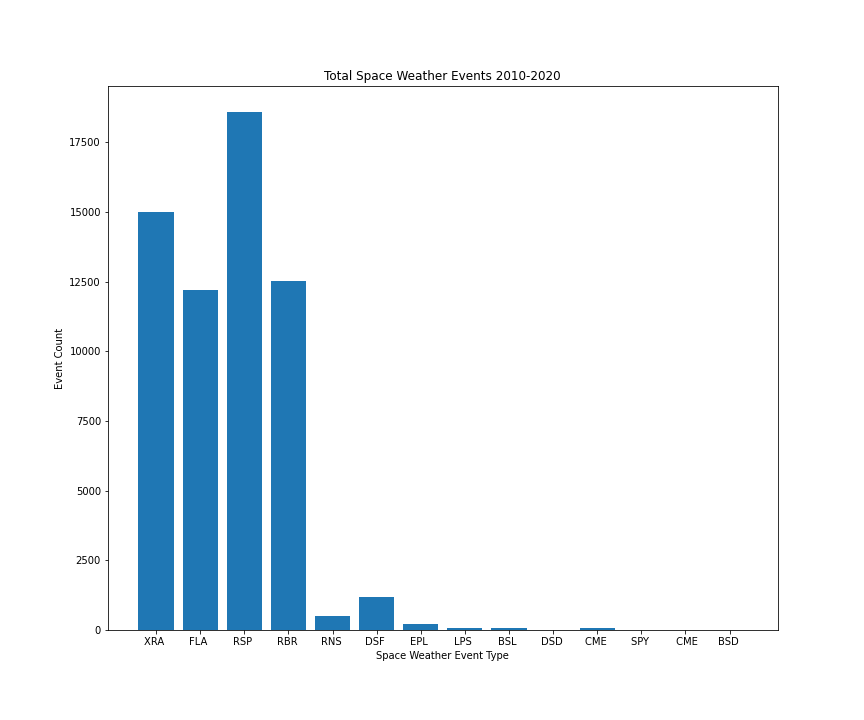
\includegraphics[width=0.75\textwidth]{figures/Space_Weather_Plot.png}
    \centering
    \caption{Total number of space weather events observed since 2010, grouped by event type (Event types are listed in table \ref{space_weather_events})}
    \label{swe_freq}
\end{figure}

\begin{table}[h!]
	\begin{center}
		\begin{tabular}{||c | c ||} 
			\hline
			Acronym & Full Name \\ [0.5ex] 
			\hline\hline
			BSL & Bright Surge on Limb \\
			\hline
			DSF & Filament Disappearance \\ 
			\hline
			EPL & Eruptive Prominence on Limb\\
			\hline
			FIL & Filament\\
			\hline
			FLA & Optical Flare in H-Alpha\\
			\hline
			FOR & Forbush Decrease (CR Decrease) \\
			\hline
			GLE & Ground-Level Event (CR Increase) \\
			\hline
			LPS & Loop Prominence System\\
			\hline
			PCA & Polar Cap Absorption\\
			\hline
			RBR & Fixed-Frequency Radio Burst\\
			\hline
			RNS & Radio Noise Storm\\
			\hline
			RSP & Sweep-Frequency Radio Burst\\
			\hline
			SPY & Spray\\
			\hline
			XRA & X-ray Event \\
			\hline
		\end{tabular}
		\caption{List of Event Types tracked in space weather reports}
		\label{space_weather_events}
	\end{center}
\end{table}

\section*{Exploratory Data Analysis}
While exploring the space weather reports we have found 79.6\% of the reports since 2010 have at least one observed space weather event, and there are on average 15.0 events per day. There are significant frequency discrepancies between the different types of space weather events. As shown in Figure 1, the most common events are X-Ray events (XRA), optical flares in H-Alpha (FLA), and Sweep-Frequency Radio Bursts (RSP), and Fixed-Frequency Radio Bursts (RBR). Each of these events comprise almost a quarter of the dataset. Because each of these four weather types have thousands of observed events to use in our CNNs, and the remaining types have at most hundreds of observed events, we have decided to focus primarily on these four types of events for this project. 

Another key feature that we have identified in the data is the typical size of a visible space weather event. Most flares and prominences are on the order of about 100 pixels in each dimension, as shown in Figure \ref{event_size}. This is good because it should allow us to down sample our images considerably from their original size of 4096x4096 pixels, which would be challenging to run through a CNN. 

\begin{figure}[h]
	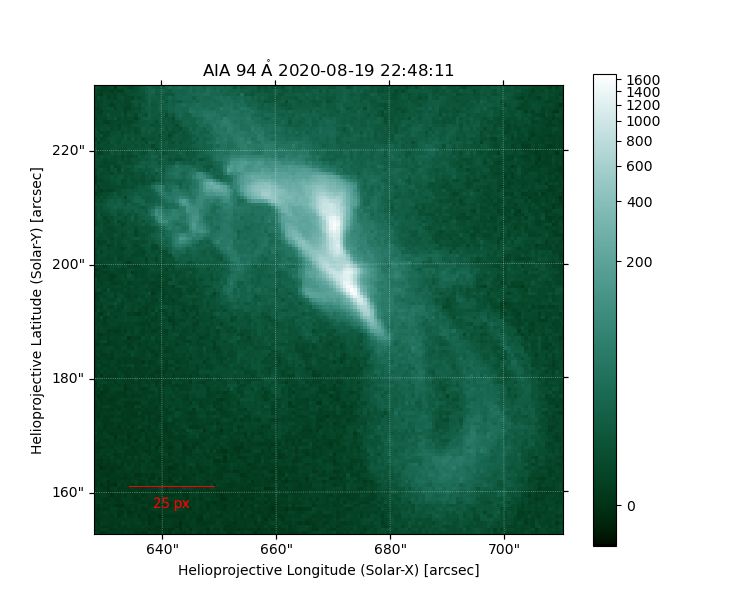
\includegraphics[width=0.8\textwidth]{figures/feature_scale.png}
	\centering
	\caption{Typical scale for an x-ray flare.}
	\label{event_size}
\end{figure}


\section*{Project Objectives}

Our project objectives fall under one major task with multiple subtasks, and two more possible objectives depending on our success.

First, we will attempt to train a neural network to identify solar events from solar images, using historical SDO AIA solar images in 5-6 wavebands between 90 and 300 Angstroms alongside solar event reports obtained from NOAA’s Space Weather Prediction Center. The images and solar event reports will be aligned in time, so that the neural network will learn to associate features within the images with specific types of solar events. We will initially focus on two types of events, x-ray events and optical flares. These events are visible in the wavelengths available to us from AIA, and they are the most frequent events in the dataset, aside from the radio burst events. 

After creating a model for identifying x-ray and optical flare events, we will apply this same methodology to radio bursts. Identifying these events with our available wavelengths is a more difficult task, because these events peak at wavelengths far outside our available range. We will attempt to use the longest wavelengths available to us on the AIA, but radio emission is well outside of the low-frequency limit of the accessible bandpasses. However, we will still train a neural network on similar sets of AIA images alongside simultaneous radio burst reports. If radio bursts carry signature features present in higher-frequency wavebands, our neural network may be able to identify them. If we are unable to create a neural network which accurately identifies these radio events, that would also be an indicator that these events do not have significant activity in our range of wavelengths. 

\section*{Event Identification Pipeline}

\subsection*{Data Wrangling}

In order to generate our testing, training and validation data sets we have written python scripts which utilize the space weather reports and the sunpy python package to download and store AIA observations. These scripts download one observation per event per wavelength, for a specified event type and set of wavelengths, which are chosen at random from all the observations taken over the duration of each event which fit the specified parameters.

Each observation, as a fits file, is 12 MB in size, and we have approximately 60,000 observed events. This means that a full collection of images would require almost a full terabyte of storage space per wavelength. In addition, the large resolution of each image (4096 x 4096 pixels) is unreasonably large to be used in our CNNs. To remedy both of these challenges we have also written a script which iterates over our downloaded images, down samples them, and saves the underlying pixel value array as a compressed .gz file. The down sampling is performed as a meanpool on 8x8 arrays of pixels, reducing the resolution to 512x512 pixels, and reducing the file size to less than 1 MB. The down sampling script is quite fast, but the image downloading script is quite slow and is the rate limiting step in this process. At the moment it takes about 60-70 seconds to download one image through google colab, compared to about 50-60 seconds per image on a local jupyter notebook connected to the Rice wifi, so building up a substantial dataset of thousands of images currently takes considerable time.


\subsection*{Modeling and Validation}

To achieve our goal of identifying solar events from AIA images, we will create a convolutional neural network using Keras, which is available in python and more user friendly than other deep learning libraries such as TensorFlow, which Keras is built on. We will create a CNN within Keras which identifies whether a solar event is present within a given image. After downsampling the observations to 512x512 pixels, the dataset of images can then be input into the neural network as numpy arrays with the number of channels used being equal to the number of wavelengths used. We will test the network subject to different parameters to discover the network design which produces the model best able to accurately identify solar events. We will modify things within the network design such as the learning rate, the batch size, and the number of convolution and pooling layers. We will test the effect of modifying these parameters by comparing the cross entropy between the different network designs.

We will validate the success of our model by setting aside one third of our dataset in each event category for three stages: training, testing, and validation. By partitioning data outside that which is used for forming the CNN, we will be able to avoid validating and testing our models on potentially overfitted data that could misrepresent the actual veracity of our model. For all CNN models, we will examine key parameters such as false positive and false negative rates in order to comprehensively evaluate their successes and shortcomings.

\subsection*{Communication}
Upon completion of our work at the end of the semester, we will present our results in an oral presentation to the course as well as in a comprehensive final report detailing our progress, results, and the potential for future work. We will also present our findings at the Rice University Data-to-Knowledge (D2K) showcase both orally and in a poster session scheduled for December 15, 2021. 




\bibliographystyle{unsrt}
\bibliography{bibfile}
\pagebreak
\section*{Appendix}


\begin{figure}[ht]
    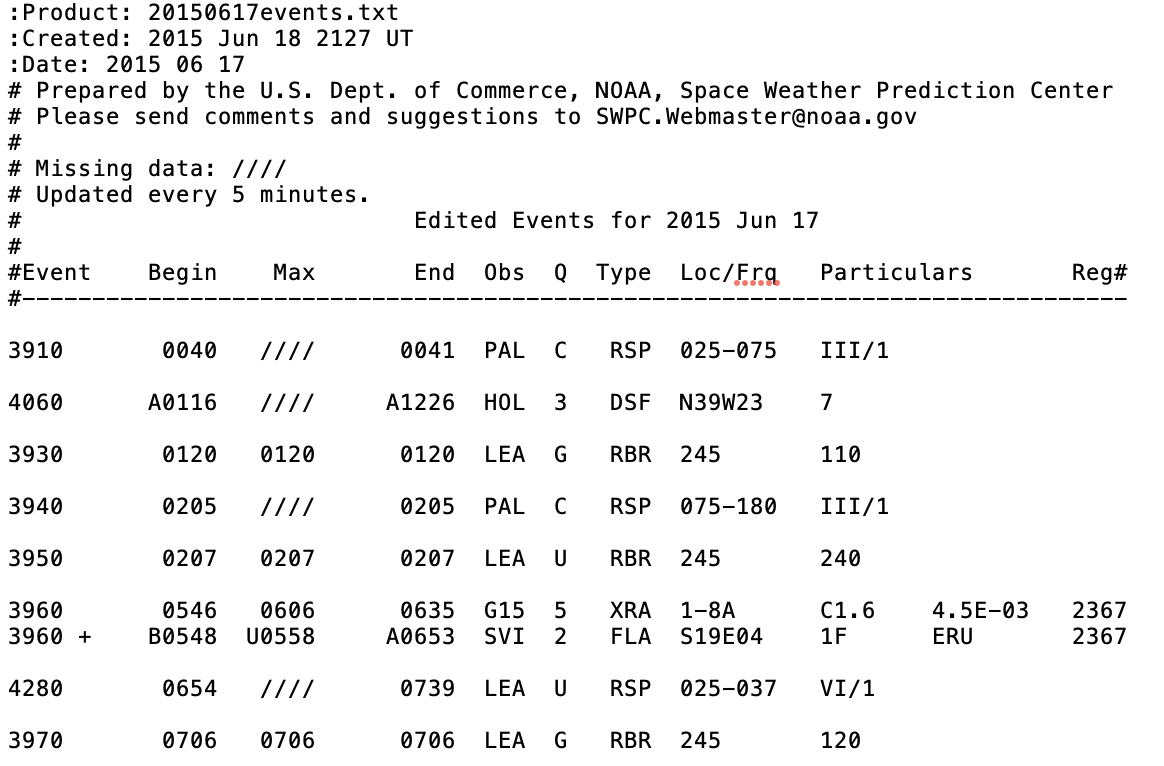
\includegraphics[width=0.9\textwidth]{figures/swr_sample.png}
    \centering
    \caption{Sample Space Weather Report text file From June 6, 2015. Along with event types and times, the reports also contain information about the event strengths and locations.}
    \label{swr_sample}
\end{figure}

\begin{figure}[ht]
	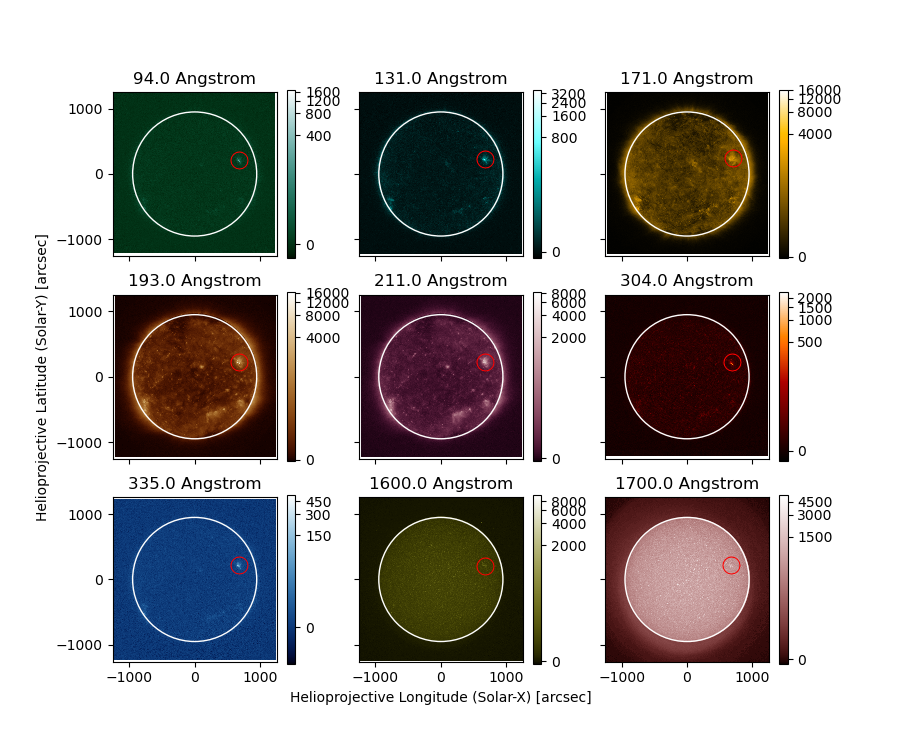
\includegraphics[width=0.9\textwidth]{figures/0819_flare_labeled.png}
	\centering
	\caption{A small x-ray flare which occurred August 19, 2020 in each AIA wavelength apart from 4500~\AA{}. The flare, circled in red on each image, shows up in all wavelengths to varying degrees.}
	\label{flare}
\end{figure}

\begin{figure}[ht]
	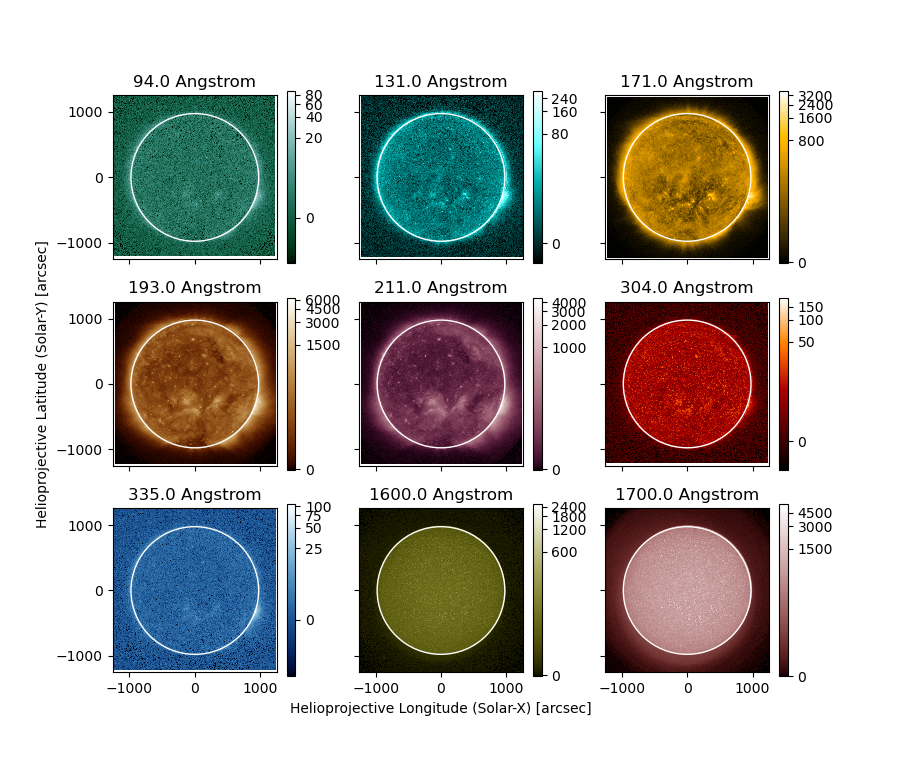
\includegraphics[width=0.9\textwidth]{figures/noflare.png}
	\centering
	\caption{The Sun in each wavelength without an active flare. Note the much smaller colorbar scales than in the image above.}
	\label{noflare}
\end{figure}

\begin{figure}[ht]
	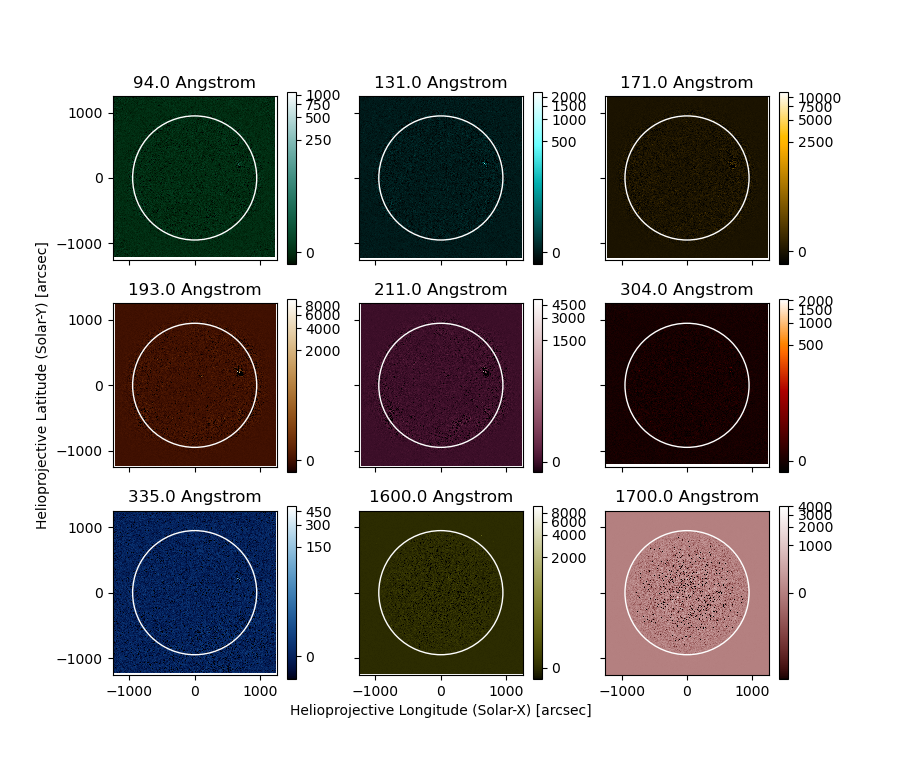
\includegraphics[width=0.9\textwidth]{figures/0819_flare_diff.png}
	\centering
	\caption{The same flare as in Figure \ref{flare} above, after subtracting a previous image from the current one. This process is sometimes called difference imaging, and is useful in seeing how an object changes over time, such as the appearance of a flare. These difference images were taken over a span of two minutes, but varying this time could optimize our detection process. The changing granulation pattern is especially apparent in the 1700~\AA{} image, where the flare is completely drowned out.}
	\label{flare_diff}
\end{figure}


\end{document}
